\chapter{KIỂM THỬ VÀ TRIỂN KHAI HỆ THỐNG}
\section{Kiểm thử hệ thống}

\subsection{Mục tiêu kiểm thử}
Đảm bảo các chức năng chính của hệ thống BarberGo hoạt động chính xác, ổn định và đáp ứng yêu cầu người dùng.

\subsection{Phạm vi kiểm thử}

\subsubsection{Mobile App - Người dùng}
\begin{itemize}
    \item Đặt lịch cắt tóc
    \item Tạo gợi ý kiểu tóc bằng AI Stable Diffusion 1.5
    \item Phát hiện mụn trên khuôn mặt với CNN và Mediapipe
    \item Chatbot tư vấn với RAG
    \item Đăng ký nâng cấp tài khoản chủ tiệm
\end{itemize}

\subsubsection{Mobile App - Chủ tiệm}
\begin{itemize}
    \item Quản lý lịch hẹn và lịch làm việc
    \item Cập nhật thông tin tiệm và dịch vụ
    \item Cập nhật vị trí tiệm trên bản đồ
\end{itemize}

\subsubsection{Web Admin}
\begin{itemize}
    \item Quản lý chủ tiệm và người dùng
    \item Chỉnh sửa prompt chatbot
\end{itemize}

\subsection{Phương pháp kiểm thử}

\begin{table}[H]
\centering
\caption{Phương pháp kiểm thử hệ thống}
\begin{tabular}{|l|p{0.35\textwidth}|l|}
\hline
\textbf{Loại} & \textbf{Mục đích} & \textbf{Công cụ} \\
\hline
Unit Testing & Kiểm thử từng module riêng lẻ & Flutter Test \\
\hline
API Testing & Kiểm thử các endpoint & Postman \\
\hline
Integration Testing & Kiểm thử tích hợp module & Postman \\
\hline
AI Model Testing & Kiểm thử độ chính xác model & Python \\
\hline
\end{tabular}
\end{table}

\subsection{Kiểm thử Model AI phát hiện mụn}

Model CNN được huấn luyện để phát hiện mụn trên khuôn mặt người dùng, kết hợp với Mediapipe để xác định vùng khuôn mặt.

\subsubsection{Thông số huấn luyện}
\begin{itemize}
    \item Mô hình MobileNetV2 (Transfer Learning), ảnh đầu vào 224×224
    \item Tập dữ liệu 4,770 ảnh, chia train/validation
    \item Huấn luyện 50 epochs với AdamW và Binary Cross Entropy
\end{itemize}


\subsubsection{Kết quả huấn luyện}

\begin{table}[H]
\centering
\caption{Kết quả huấn luyện Model CNN theo epoch}
\begin{tabular}{|c|c|c|c|c|}
\hline
\textbf{Epoch} & \textbf{Train Loss} & \textbf{Train Acc} & \textbf{Val Loss} & \textbf{Val Acc} \\
\hline
1 & 0.0784 & 0.9750 & 0.0131 & 0.9953 \\
\hline
5 & 0.0101 & 0.9973 & 0.0007 & 1.0000 \\
\hline
10 & 0.0088 & 0.9973 & 0.0006 & 1.0000 \\
\hline
15 & 0.0020 & 0.9994 & 0.0009 & 1.0000 \\
\hline
20 & 0.0007 & 0.9996 & 0.0001 & 1.0000 \\
\hline
25 & 0.0007 & 0.9997 & 0.0001 & 1.0000 \\
\hline
30 & 0.0008 & 0.9997 & 0.0001 & 1.0000 \\
\hline
35 & 0.0009 & 0.9999 & 0.0000 & 1.0000 \\
\hline
40 & 0.0017 & 0.9997 & 0.0001 & 1.0000 \\
\hline
45 & 0.0017 & 0.9999 & 0.0000 & 1.0000 \\
\hline
50 & 0.0011 & 0.9997 & 0.0001 & 1.0000 \\
\hline
\end{tabular}
\end{table}

\subsection{Biểu đồ kết quả huấn luyện Model CNN}
\begin{figure}[H]
    \centering
    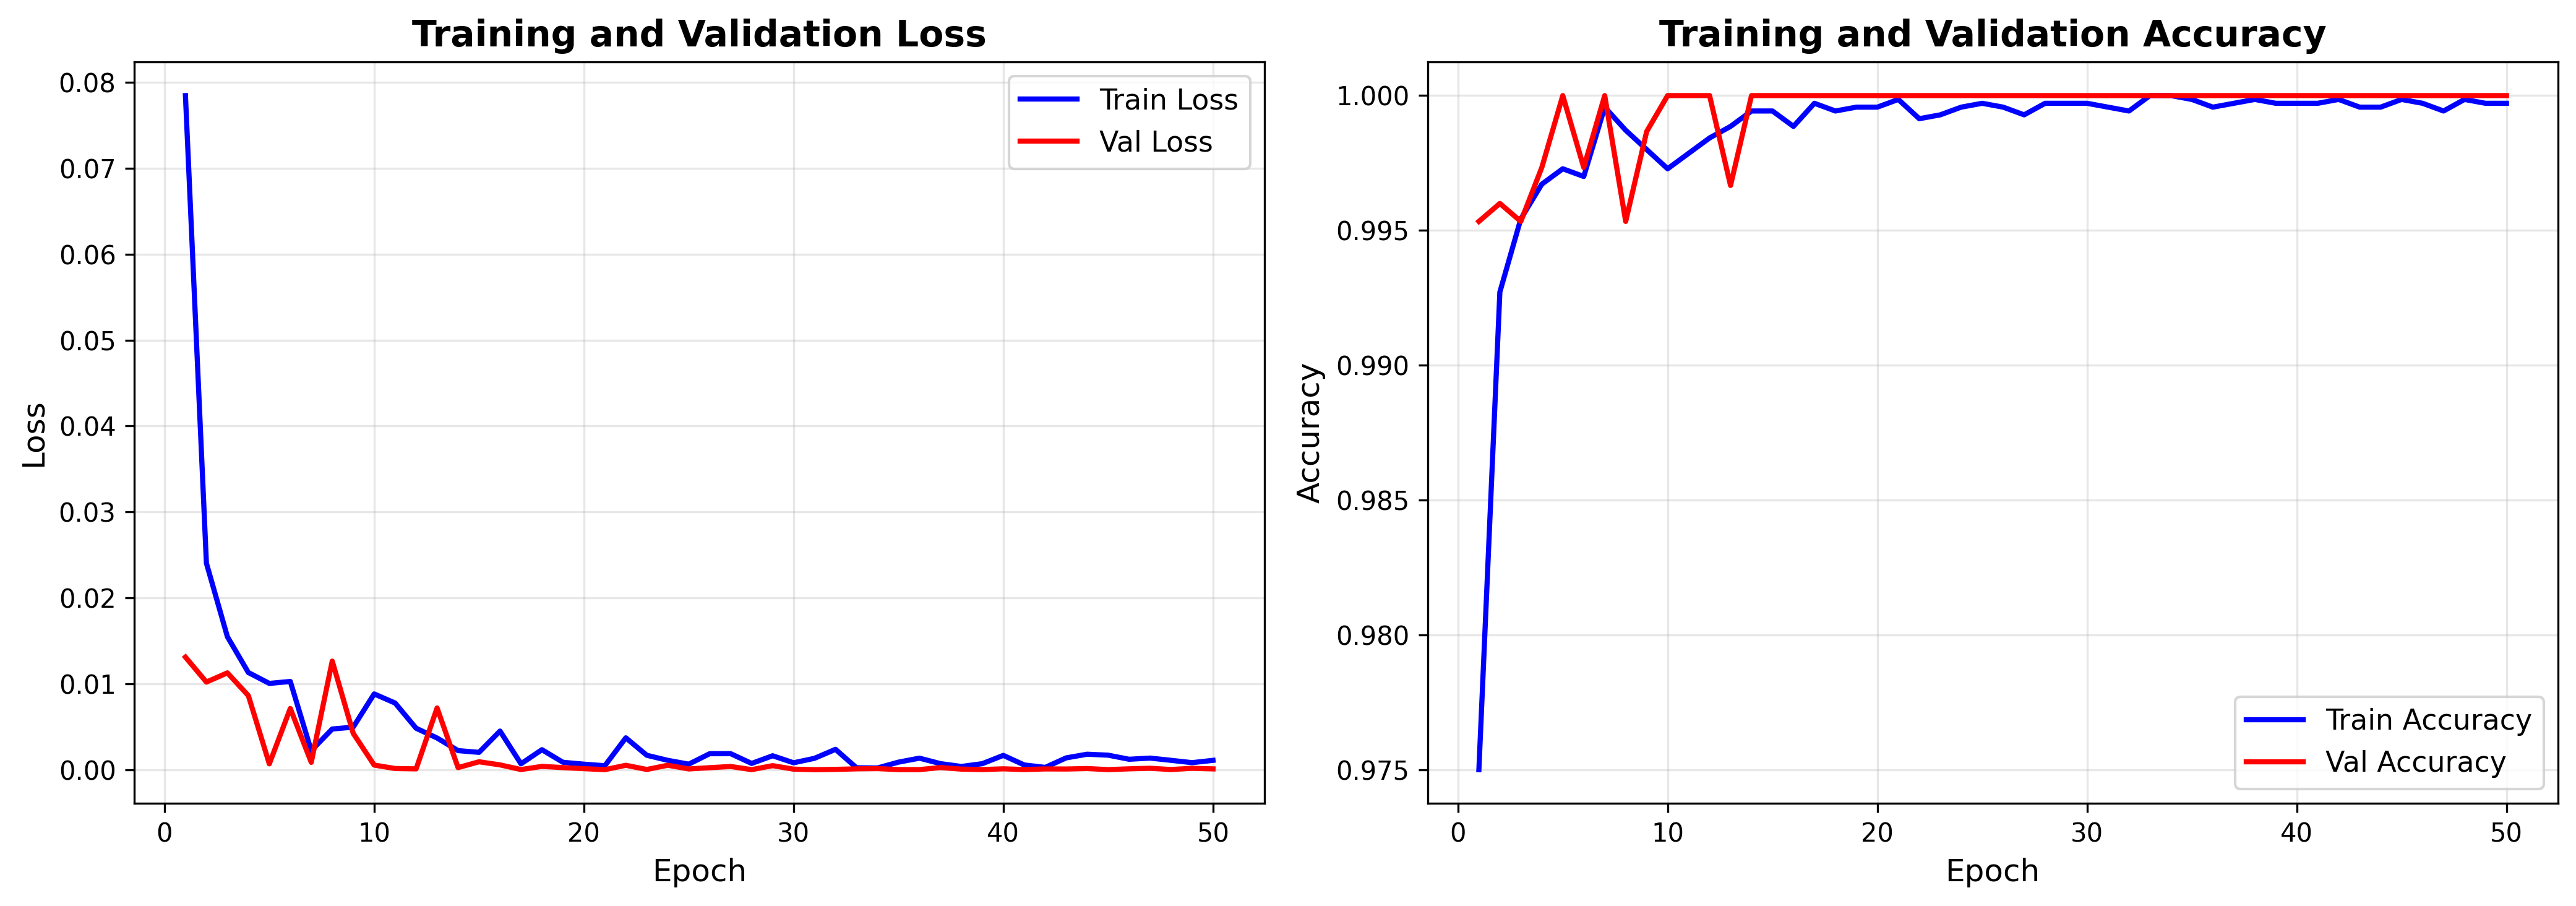
\includegraphics[width=1.0\textwidth]{figures/training_chart.png}
    \caption{Biểu đồ kết quả huấn luyện Model CNN}
    \label{fig:training_chart}
\end{figure}
\subsubsection{Đánh giá kết quả}

Từ kết quả huấn luyện, model đạt được:
\begin{itemize}
    \item Độ chính xác trên tập validation: 100\% (từ epoch 5 trở đi)
    \item Loss giảm nhanh và ổn định sau epoch 20
    \item Không có dấu hiệu overfitting nghiêm trọng
    \item Thời gian inference: dưới 3 giây
\end{itemize}

Model cho thấy khả năng phân loại tốt giữa ảnh có mụn và không có mụn, phù hợp để tích hợp vào ứng dụng thực tế.

\subsection{Kiểm thử API}

\subsubsection{Danh sách Endpoints}

Hệ thống BarberGo cung cấp các nhóm API sau:

\textbf{Authentication APIs}
\begin{itemize}
    \item POST /api/auth/register - Đăng ký tài khoản
    \item POST /api/auth/login - Đăng nhập
    \item POST /api/auth/logout - Đăng xuất
    \item POST /api/auth/refresh-token - Làm mới token
\end{itemize}

\textbf{User APIs}
\begin{itemize}
    \item GET /api/users/profile - Xem thông tin cá nhân
    \item PUT /api/users/profile - Cập nhật thông tin
    \item POST /api/users/upgrade-to-owner - Nâng cấp chủ tiệm
    \item GET /api/users/bookings - Xem lịch hẹn
\end{itemize}

\textbf{Booking APIs}
\begin{itemize}
    \item GET /api/bookings - Danh sách lịch hẹn
    \item POST /api/bookings - Tạo lịch hẹn
    \item GET /api/bookings/\{id\} - Chi tiết lịch hẹn
    \item PUT /api/bookings/\{id\} - Cập nhật lịch hẹn
    \item DELETE /api/bookings/\{id\} - Hủy lịch hẹn
\end{itemize}

\textbf{Shop APIs}
\begin{itemize}
    \item GET /api/shops - Danh sách tiệm
    \item GET /api/shops/\{id\} - Chi tiết tiệm
    \item POST /api/shops - Tạo tiệm mới
    \item PUT /api/shops/\{id\} - Cập nhật thông tin tiệm
    \item PUT /api/shops/\{id\}/location - Cập nhật vị trí
    \item GET /api/shops/\{id\}/services - Danh sách dịch vụ
    \item POST /api/shops/\{id\}/services - Thêm dịch vụ
\end{itemize}

\textbf{Schedule APIs}
\begin{itemize}
    \item GET /api/schedules - Xem lịch làm việc
    \item POST /api/schedules - Tạo lịch làm việc
    \item PUT /api/schedules/\{id\} - Cập nhật lịch
    \item DELETE /api/schedules/\{id\} - Xóa lịch
\end{itemize}

\textbf{AI APIs}
\begin{itemize}
    \item POST /api/ai/hairstyle-generate - Tạo gợi ý kiểu tóc
    \item POST /api/ai/acne-detection - Phát hiện mụn
    \item GET /api/ai/results/\{id\} - Lấy kết quả AI
\end{itemize}

\textbf{Chatbot APIs}
\begin{itemize}
    \item POST /api/chatbot/message - Gửi tin nhắn
    \item GET /api/chatbot/history - Lịch sử chat
    \item DELETE /api/chatbot/history - Xóa lịch sử
\end{itemize}

\textbf{Admin APIs}
\begin{itemize}
    \item GET /api/admin/users - Danh sách người dùng
    \item PUT /api/admin/users/\{id\}/status - Cập nhật trạng thái
    \item DELETE /api/admin/users/\{id\} - Xóa người dùng
    \item GET /api/admin/shops - Danh sách tiệm
    \item PUT /api/admin/shops/\{id\}/approve - Phê duyệt tiệm
    \item PUT /api/admin/chatbot/prompt - Cập nhật prompt
\end{itemize}

\subsubsection{Kết quả kiểm thử API}

\begin{table}[h]
\centering
\caption{Kết quả kiểm thử theo nhóm API}
\begin{tabular}{|l|c|c|}
\hline
\textbf{Nhóm API} & \textbf{Số test} & \textbf{Pass rate} \\
\hline
Authentication & 6 & 100\% \\
\hline
User Management & 8 & 100\% \\
\hline
Booking & 10 & 100\% \\
\hline
Shop & 12 & 92\% \\
\hline
AI Services & 6 & 100\% \\
\hline
Chatbot & 4 & 100\% \\
\hline
Admin & 4 & 100\% \\
\hline
\textbf{Tổng} & \textbf{50} & \textbf{96\%} \\
\hline
\end{tabular}
\end{table}

\subsubsection{Tiêu chí đánh giá}

\begin{table}[h]
\centering
\caption{Tiêu chí đánh giá hiệu năng API}
\begin{tabular}{|l|c|}
\hline
\textbf{Tiêu chí} & \textbf{Mục tiêu} \\
\hline
Tỷ lệ test Pass & $\geq$ 95\% \\
\hline
Response time (API thường) & $\leq$ 2s \\
\hline
Response time (AI Gen ảnh) & $\leq$ 10s \\
\hline
Response time (AI Phát hiện mụn) & $\leq$ 3s \\
\hline
Response time (Chatbot) & $\leq$ 2s \\
\hline
Độ chính xác Model CNN & $\geq$ 95\% \\
\hline
\end{tabular}
\end{table}

\subsection{Môi trường kiểm thử}
\begin{itemize}
    \item Mobile: Flutter 3.x (Android 10+, iOS 14+)
    \item Backend: Python Flask
    \item Web Admin: Nuxt.js 3.x
    \item Database: Supabase PostgreSQL
    \item AI Models: Stable Diffusion 1.5, MobileNetV2, Mediapipe
    \item Tools: Postman, Python
\end{itemize}

\subsection{Kết quả kiểm thử tổng hợp}

Kết quả kiểm thử cho thấy:
\begin{itemize}
    \item Tổng số test cases: 50
    \item Test Pass: 48 (96\%)
    \item Thời gian response trung bình: 1.2 giây
    \item Model CNN đạt 100\% accuracy trên tập validation
    \item Hệ thống hoạt động ổn định và đáp ứng yêu cầu
\end{itemize}


\section{Cài đặt và Triển khai}


\subsection{Môi trường triển khai}

Hệ thống BarberGo được triển khai theo mô hình client-server, bao gồm Backend API, Web Admin và Mobile App. Môi trường triển khai được tóm tắt trong Bảng~\ref{tab:environment}.

\begin{table}[H]
\centering
\caption{Môi trường triển khai hệ thống}
\label{tab:environment}
\begin{tabular}{|p{4cm}|p{9.5cm}|}
\hline
\textbf{Thành phần} & \textbf{Mô tả} \\
\hline
Server &
Ubuntu 22.04 LTS, CPU từ 4 cores, RAM 8GB (khuyến nghị 16GB), SSD 50GB, GPU NVIDIA hỗ trợ CUDA cho AI inference \\
\hline
Backend &
Flask API (Python 3.10+), triển khai với Gunicorn và Nginx \\
\hline
Web Admin &
Ứng dụng web quản trị, build và deploy trên nền tảng CDN (Vercel/Netlify) \\
\hline
Mobile App &
Ứng dụng Flutter, hỗ trợ Android và iOS \\
\hline
Database &
Supabase PostgreSQL, áp dụng Row Level Security (RLS) \\
\hline
AI Models &
Stable Diffusion 1.5 và mô hình CNN phát hiện mụn \\
\hline
\end{tabular}
\end{table}

\subsection{Triển khai hệ thống}

Backend API được triển khai trên server sử dụng Nginx làm reverse proxy nhằm tăng cường khả năng bảo mật và xử lý đồng thời. Các AI models được load khi hệ thống khởi động để phục vụ inference theo yêu cầu.

Web Admin được build thành static files và triển khai trên nền tảng CDN nhằm tối ưu tốc độ truy cập. Mobile App được build bản release và phân phối thông qua Google Play Store và Apple App Store.

\subsection{Bảo mật và vận hành}

Hệ thống áp dụng các biện pháp bảo mật bao gồm HTTPS với SSL/TLS, xác thực người dùng bằng JWT, giới hạn tần suất truy cập API và cấu hình firewall. Cơ chế backup và monitoring được thiết lập nhằm đảm bảo khả năng phục hồi và giám sát trạng thái hệ thống.


\section{Kiểm thử hệ thống}

\subsection{Mục tiêu kiểm thử}

Quá trình kiểm thử nhằm đánh giá tính đúng đắn, ổn định và khả năng hoạt động đồng bộ của các thành phần trong hệ thống BarberGo sau khi triển khai.

\subsection{Kiểm thử chức năng}

Các chức năng chính của hệ thống được kiểm thử bao gồm xác thực người dùng, quản lý lịch hẹn, kết nối cơ sở dữ liệu, xử lý AI và giao tiếp giữa Mobile App, Web Admin với Backend API.

\subsection{Kiểm thử sau triển khai}

Kết quả kiểm thử tổng hợp được trình bày trong Bảng~\ref{tab:testing}.

\begin{table}[H]
\centering
\caption{Kết quả kiểm thử sau triển khai}
\label{tab:testing}
\begin{tabular}{|p{8cm}|c|}
\hline
\textbf{Hạng mục kiểm thử} & \textbf{Kết quả} \\
\hline
Backend API hoạt động ổn định & Đạt \\
\hline
Kết nối cơ sở dữ liệu Supabase & Đạt \\
\hline
AI models load và inference & Đạt \\
\hline
Web Admin kết nối Backend & Đạt \\
\hline
Mobile App giao tiếp API & Đạt \\
\hline
Bảo mật SSL/TLS & Đạt \\
\hline
Logging và monitoring & Đạt \\
\hline
\end{tabular}
\end{table}

\subsection{Đánh giá}

Kết quả kiểm thử cho thấy hệ thống BarberGo đáp ứng đầy đủ các yêu cầu chức năng và phi chức năng đã đề ra. Hệ thống hoạt động ổn định, đảm bảo tính bảo mật và sẵn sàng cho môi trường production.
